% ===========================================================================
%  TikuOS — Timer Subsystem: Clock, Software Timers & Hardware Timers
%  Beamer Presentation
% ===========================================================================
\documentclass[aspectratio=169, 10pt]{beamer}

% ---- Theme ----------------------------------------------------------------
\usetheme{Madrid}
\usecolortheme{whale}
\setbeamertemplate{navigation symbols}{}
\setbeamertemplate{footline}{%
  \leavevmode\hbox{%
    \begin{beamercolorbox}[wd=.33\paperwidth,ht=2.5ex,dp=1ex,center]{author in head/foot}%
      \usebeamerfont{author in head/foot}\insertshortauthor
    \end{beamercolorbox}%
    \begin{beamercolorbox}[wd=.34\paperwidth,ht=2.5ex,dp=1ex,center]{title in head/foot}%
      \usebeamerfont{title in head/foot}\insertshorttitle
    \end{beamercolorbox}%
    \begin{beamercolorbox}[wd=.33\paperwidth,ht=2.5ex,dp=1ex,right]{date in head/foot}%
      \usebeamerfont{date in head/foot}\insertshortdate{}\hspace*{2em}%
      \insertframenumber{}/\inserttotalframenumber\hspace*{2ex}
    \end{beamercolorbox}}%
  \vskip0pt%
}

% ---- Packages -------------------------------------------------------------
\usepackage{listings}
\usepackage{graphicx}
\usepackage{hyperref}
\usepackage{booktabs}
\usepackage{multirow}
\usepackage{tikz}
\usetikzlibrary{arrows.meta, positioning, shapes.geometric, calc,
                decorations.pathreplacing, fit}

% ---- Code listing style ---------------------------------------------------
\lstset{
  basicstyle=\ttfamily\scriptsize,
  keywordstyle=\color{blue}\bfseries,
  commentstyle=\color{gray},
  stringstyle=\color{red!70!black},
  showstringspaces=false,
  breaklines=true,
  frame=single,
  rulecolor=\color{black!30},
  backgroundcolor=\color{blue!3},
  tabsize=4,
}
\lstdefinestyle{cstyle}{
  language=C,
  morekeywords={uint8_t,uint16_t,uint32_t,
                tiku_clock_time_t,tiku_clock_arch_time_t,
                tiku_htimer_clock_t,tiku_htimer_callback_t,
                tiku_timer_callback_t,tiku_timer_mode,
                TIKU_CLOCK_SECOND,TIKU_HTIMER_SECOND,
                TIKU_HTIMER_NOW,TIKU_HTIMER_TIME,
                TIKU_HTIMER_OK,TIKU_HTIMER_ERR_TIME,
                TIKU_HTIMER_ERR_INVALID,TIKU_HTIMER_ERR_NONE,
                TIKU_TIMER_MODE_EVENT,TIKU_TIMER_MODE_CALLBACK,
                TIKU_EVENT_TIMER,TIKU_EVENT_POLL,
                TIKU_PROCESS,TIKU_PROCESS_THREAD,
                TIKU_PROCESS_BEGIN,TIKU_PROCESS_END,
                TIKU_PROCESS_WAIT_EVENT,TIKU_PROCESS_WAIT_EVENT_UNTIL,
                TIKU_AUTOSTART_PROCESSES,TIKU_CLOCK_MS_TO_TICKS,
                TIKU_ISR,NULL},
}

% ---- Metadata -------------------------------------------------------------
\title[TikuOS Timers]{TikuOS Timer Subsystem}
\subtitle{Simple. Ubiquitous. Intelligence, Everywhere.}
\author[Ambuj Varshney]{Ambuj Varshney \\ \texttt{ambuj@tiku-os.org}}
\date{\today}

% ===========================================================================
\begin{document}

% ---------------------------------------------------------------------------
\begin{frame}
\titlepage
\end{frame}

% ---------------------------------------------------------------------------
\begin{frame}{Outline}
\tableofcontents
\end{frame}

% ===========================================================================
\section{Timer Architecture}
% ===========================================================================

\begin{frame}[fragile]{Three-Layer Timer Design}
\begin{center}
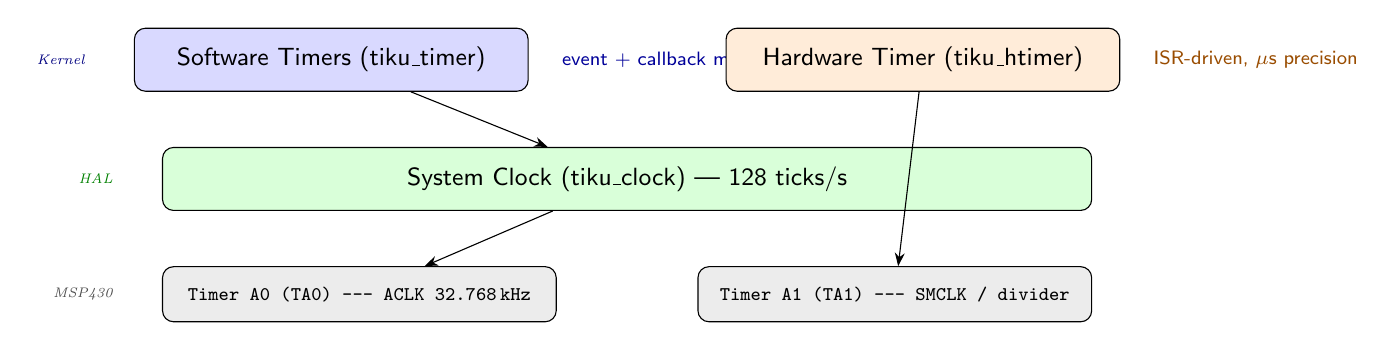
\begin{tikzpicture}[
    box/.style={draw, rounded corners, minimum height=0.8cm,
                text centered, font=\small\sffamily, fill=#1},
    hw/.style={draw, rounded corners, minimum height=0.7cm,
               text centered, font=\scriptsize\ttfamily, fill=gray!15},
    >=Stealth, node distance=0.5cm
  ]

  % Software Timer layer
  \node[box=blue!15, minimum width=5cm] (stimer)
    {Software Timers (tiku\_timer)};
  \node[right=0.3cm of stimer, font=\scriptsize\sffamily, text=blue!60!black]
    {event + callback modes};

  % Hardware Timer layer
  \node[box=orange!15, minimum width=5cm, right=2.5cm of stimer] (htimer)
    {Hardware Timer (tiku\_htimer)};
  \node[right=0.3cm of htimer, font=\scriptsize\sffamily, text=orange!60!black]
    {ISR-driven, $\mu$s precision};

  % System Clock layer
  \node[box=green!15, minimum width=11.8cm, below=0.7cm of $(stimer.south)!0.5!(htimer.south)$] (clock)
    {System Clock (tiku\_clock) --- 128 ticks/s};

  % Arch layer
  \node[hw, minimum width=5cm, below=0.7cm of clock.south west, anchor=north west] (ta0)
    {Timer A0 (TA0) --- ACLK 32.768\,kHz};
  \node[hw, minimum width=5cm, below=0.7cm of clock.south east, anchor=north east] (ta1)
    {Timer A1 (TA1) --- SMCLK / divider};

  % Arrows
  \draw[->] (stimer) -- (clock);
  \draw[->] (htimer) -- (ta1);
  \draw[->] (clock) -- (ta0);

  % Labels
  \node[left=0.5cm of stimer, font=\tiny\itshape, text=blue!50!black] {Kernel};
  \node[left=0.5cm of clock, font=\tiny\itshape, text=green!50!black] {HAL};
  \node[left=0.5cm of ta0, font=\tiny\itshape, text=gray!60!black] {MSP430};

\end{tikzpicture}
\end{center}

\vspace{0.3em}
\begin{table}
\centering
\small
\begin{tabular}{@{}lccc@{}}
\toprule
& \textbf{System Clock} & \textbf{Software Timer} & \textbf{Hardware Timer} \\
\midrule
Resolution   & 7.8\,ms (128\,Hz) & 7.8\,ms & 1\,$\mu$s (configurable) \\
Concurrency  & --- & Multiple (linked list) & Single (one pending) \\
Context      & ISR & Timer process & ISR \\
Use case     & Timekeeping & Process events/callbacks & Precise ISR timing \\
\bottomrule
\end{tabular}
\end{table}
\end{frame}

% ===========================================================================
\section{System Clock}
% ===========================================================================

\begin{frame}[fragile]{System Clock Configuration}
\begin{columns}[T]
\begin{column}{0.48\textwidth}
\begin{lstlisting}[style=cstyle,
  title={arch/msp430/tiku\_timer\_arch.h}]
/* Ticks per second (power of 2) */
#define TIKU_CLOCK_ARCH_SECOND  128

/* ACLK from XT1 crystal */
#define TIKU_CLOCK_ARCH_ACLK_FREQ \
    32768

/* ISR fires every 256 ACLK ticks */
#define TIKU_CLOCK_ARCH_INTERVAL \
    (32768 / 128)  /* = 256 */
\end{lstlisting}

\begin{lstlisting}[style=cstyle, title={Clock types}]
typedef unsigned short
    tiku_clock_time_t;      /* 16-bit */
typedef unsigned long
    tiku_clock_arch_time_t; /* 32-bit */
\end{lstlisting}
\end{column}

\begin{column}{0.48\textwidth}
\textbf{How it works:}
\begin{enumerate}
  \item Timer A0 runs from ACLK (32.768\,kHz crystal)
  \item CCR0 compare interrupt fires every 256 ACLK cycles
  \item ISR increments tick counter (128 ticks/s)
  \item Every 128 ticks, seconds counter increments
  \item ISR wakes CPU from LPM3
\end{enumerate}

\vspace{0.3em}
\begin{block}{TIKU\_CLOCK\_SECOND}
Convenience macro = 128.\\
One second = 128 ticks.\\
Half second = \texttt{TIKU\_CLOCK\_SECOND / 2}.
\end{block}
\end{column}
\end{columns}
\end{frame}

% ---------------------------------------------------------------------------
\begin{frame}[fragile]{Clock API}
\begin{table}
\centering
\small
\begin{tabular}{@{}lp{7.5cm}@{}}
\toprule
\textbf{Function / Macro} & \textbf{Description} \\
\midrule
\texttt{tiku\_clock\_init()}      & Start Timer A0, enable interrupts \\
\texttt{tiku\_clock\_time()}      & Current tick count (16-bit, wraps) \\
\texttt{tiku\_clock\_seconds()}   & Elapsed seconds since boot \\
\texttt{tiku\_clock\_wait(t)}     & Busy-wait for \texttt{t} ticks \\
\texttt{tiku\_clock\_delay\_usec(dt)} & Microsecond-scale busy delay \\
\midrule
\texttt{TIKU\_CLOCK\_SECOND}        & Ticks per second (128) \\
\texttt{TIKU\_CLOCK\_MS\_TO\_TICKS(ms)} & Convert milliseconds to ticks \\
\texttt{TIKU\_CLOCK\_LT(a,b)}       & Wraparound-safe \texttt{a < b} \\
\texttt{TIKU\_CLOCK\_DIFF(a,b)}     & Wraparound-safe \texttt{a - b} \\
\bottomrule
\end{tabular}
\end{table}

\vspace{0.3em}
\begin{alertblock}{Wraparound Safety}
The 16-bit tick counter wraps every \textasciitilde512 seconds.
\textbf{Always} use \texttt{TIKU\_CLOCK\_LT()} and \texttt{TIKU\_CLOCK\_DIFF()}
for comparisons --- never raw \texttt{<} or \texttt{-}.
\end{alertblock}
\end{frame}

% ---------------------------------------------------------------------------
\begin{frame}[fragile]{Clock ISR \& Atomic Reads}
\begin{columns}[T]
\begin{column}{0.48\textwidth}
\begin{lstlisting}[style=cstyle, title={Timer A0 ISR (simplified)}]
TIKU_ISR(TIMER0_A0_VECTOR,
         timer0_a0_isr)
{
    tiku_arch_last_tar = TA0R;
    ++tiku_arch_count;

    if ((tiku_arch_count %
         TIKU_CLOCK_ARCH_SECOND) == 0)
        ++tiku_arch_seconds;

    /* Wake timer process */
    tiku_timer_request_poll();

    /* Exit LPM3 */
    __bic_SR_register_on_exit(
        LPM3_bits);
}
\end{lstlisting}
\end{column}

\begin{column}{0.48\textwidth}
\begin{lstlisting}[style=cstyle, title={Double-read for stability}]
tiku_clock_arch_time_t
tiku_clock_arch_time(void)
{
    tiku_clock_arch_time_t t1, t2;
    do {
        t1 = tiku_arch_count;
        t2 = tiku_arch_count;
    } while (t1 != t2);
    return t1;
}
\end{lstlisting}

\vspace{0.3em}
\begin{block}{Why Double-Read?}
On 16-bit MSP430, a 32-bit read
is not atomic. ISR can fire between
the two 16-bit loads.
Repeat until stable.
\end{block}
\end{column}
\end{columns}
\end{frame}

% ===========================================================================
\section{Software Timers}
% ===========================================================================

\begin{frame}[fragile]{Timer Structure \& Modes}
\begin{columns}[T]
\begin{column}{0.50\textwidth}
\begin{lstlisting}[style=cstyle,
  title={kernel/timers/tiku\_timer.h}]
struct tiku_timer {
    struct tiku_timer *next;
    tiku_clock_time_t  start;
    tiku_clock_time_t  interval;
    uint8_t  mode;     /* EVENT or CB */
    uint8_t  active;
    struct tiku_process *p;
    tiku_timer_callback_t func;
    void *ptr;
};
\end{lstlisting}

\textbf{Expiration check:}
\begin{lstlisting}[style=cstyle]
static inline int timer_is_due(
    struct tiku_timer *t,
    tiku_clock_time_t now)
{
    return (tiku_clock_time_t)
        (now - t->start) >= t->interval;
}
\end{lstlisting}
\end{column}

\begin{column}{0.46\textwidth}
\textbf{Two operating modes:}

\vspace{0.3em}
\begin{block}{Event Mode}
Posts \texttt{TIKU\_EVENT\_TIMER} to the
owning process when expired.\\
Process waits with\\
\texttt{WAIT\_EVENT\_UNTIL(ev == TIMER)}.
\end{block}

\begin{block}{Callback Mode}
Calls a function directly when expired.\\
Runs in the timer management process context.\\
No need to write a process for simple periodic work.
\end{block}

\vspace{0.3em}
\textasciitilde24 bytes per timer instance.\\
All statically allocated.
\end{column}
\end{columns}
\end{frame}

% ---------------------------------------------------------------------------
\begin{frame}[fragile]{Event Timer API}
\begin{lstlisting}[style=cstyle, title={Set an event timer}]
static struct tiku_timer my_timer;

/* Start a 1-second timer (posts TIKU_EVENT_TIMER to calling process) */
tiku_timer_set_event(&my_timer, TIKU_CLOCK_SECOND);
\end{lstlisting}

\begin{lstlisting}[style=cstyle, title={Wait for the timer event}]
TIKU_PROCESS_WAIT_EVENT_UNTIL(ev == TIKU_EVENT_TIMER);
/* Timer has fired --- do work */
\end{lstlisting}

\begin{lstlisting}[style=cstyle, title={Periodic: drift-free reset}]
while (1) {
    TIKU_PROCESS_WAIT_EVENT_UNTIL(ev == TIKU_EVENT_TIMER);
    tiku_common_led1_toggle();
    tiku_timer_reset(&my_timer);   /* start += interval (no drift) */
}
\end{lstlisting}

\begin{alertblock}{reset() vs restart()}
\texttt{tiku\_timer\_reset()} --- advances \texttt{start} by \texttt{interval} (drift-free).\\
\texttt{tiku\_timer\_restart()} --- sets \texttt{start = now} (accumulates drift).\\
Use \texttt{reset()} for periodic timers.
\end{alertblock}
\end{frame}

% ---------------------------------------------------------------------------
\begin{frame}[fragile]{Callback Timer API}
\begin{lstlisting}[style=cstyle, title={Set a callback timer}]
static struct tiku_timer cb_timer;

void my_callback(void *ptr) {
    tiku_common_led1_toggle();
    tiku_timer_reset(&cb_timer);   /* reschedule for periodic */
}

/* Start 500ms callback timer */
tiku_timer_set_callback(&cb_timer, TIKU_CLOCK_SECOND / 2,
                        my_callback, NULL);
\end{lstlisting}

\vspace{0.3em}
\begin{columns}[T]
\begin{column}{0.48\textwidth}
\begin{block}{When to Use Callbacks}
\begin{itemize}
  \item Simple periodic actions (LED toggle)
  \item No need for a full process
  \item Multiple independent timers
  \item Self-rescheduling with \texttt{reset()}
\end{itemize}
\end{block}
\end{column}
\begin{column}{0.48\textwidth}
\begin{block}{When to Use Event Timers}
\begin{itemize}
  \item Process already exists
  \item Need to combine with other events
  \item Timeout patterns
  \item Complex state machines
\end{itemize}
\end{block}
\end{column}
\end{columns}
\end{frame}

% ---------------------------------------------------------------------------
\begin{frame}[fragile]{Timer Control Functions}
\begin{table}
\centering
\small
\begin{tabular}{@{}lp{8cm}@{}}
\toprule
\textbf{Function} & \textbf{Description} \\
\midrule
\texttt{tiku\_timer\_set\_event(t, ticks)}     & Start event timer for calling process \\
\texttt{tiku\_timer\_set\_callback(t, ticks, fn, ptr)} & Start callback timer \\
\texttt{tiku\_timer\_reset(t)}                 & Drift-free reschedule: \texttt{start += interval} \\
\texttt{tiku\_timer\_restart(t)}               & Reschedule from now: \texttt{start = now} \\
\texttt{tiku\_timer\_stop(t)}                  & Cancel timer, remove from active list \\
\midrule
\texttt{tiku\_timer\_expired(t)}               & True if timer is not active \\
\texttt{tiku\_timer\_remaining(t)}             & Ticks until expiration \\
\texttt{tiku\_timer\_expiration\_time(t)}       & Absolute tick of expiration \\
\midrule
\texttt{tiku\_timer\_any\_pending()}            & True if any timer is active \\
\texttt{tiku\_timer\_next\_expiration()}        & Nearest expiration tick \\
\bottomrule
\end{tabular}
\end{table}
\end{frame}

% ---------------------------------------------------------------------------
\begin{frame}[fragile]{Timer Management Internals}
\begin{columns}[T]
\begin{column}{0.52\textwidth}
\textbf{How software timers are dispatched:}
\begin{enumerate}
  \item Clock ISR fires every 7.8\,ms
  \item ISR calls \texttt{tiku\_timer\_request\_poll()}
  \item Timer management process wakes
  \item Walks linked list of active timers
  \item For each due timer:
    \begin{itemize}
      \item \textbf{Event mode}: post \texttt{TIKU\_EVENT\_TIMER}
      \item \textbf{Callback mode}: call \texttt{func(ptr)}
    \end{itemize}
  \item Expired timers removed from list
  \item List rescanned after each dispatch\\
        (callbacks may modify the list)
\end{enumerate}
\end{column}

\begin{column}{0.44\textwidth}
\begin{lstlisting}[style=cstyle, basicstyle=\ttfamily\tiny,
  title={Timer process (simplified)}]
TIKU_PROCESS_THREAD(
    tiku_timer_process, ev, data)
{
    TIKU_PROCESS_BEGIN();

    while (1) {
        TIKU_PROCESS_WAIT_EVENT();

        if (ev == TIKU_EVENT_POLL) {
            /* Walk timer list */
            now = tiku_clock_time();
            for each active timer t:
                if timer_is_due(t, now):
                    dispatch(t);
        }
        if (ev == TIKU_EVENT_EXITED)
            /* Cleanup dead process
               timers */
    }

    TIKU_PROCESS_END();
}
\end{lstlisting}
\end{column}
\end{columns}
\end{frame}

% ===========================================================================
\section{Hardware Timer (htimer)}
% ===========================================================================

\begin{frame}[fragile]{Hardware Timer: Microsecond Precision}
\begin{columns}[T]
\begin{column}{0.48\textwidth}
\begin{lstlisting}[style=cstyle,
  title={kernel/timers/tiku\_htimer.h}]
struct tiku_htimer {
    tiku_htimer_clock_t time;
    tiku_htimer_callback_t func;
    void *ptr;
};

/* Callback signature */
typedef void (*tiku_htimer_callback_t)(
    struct tiku_htimer *t, void *ptr);
\end{lstlisting}

\begin{lstlisting}[style=cstyle, title={Status codes}]
TIKU_HTIMER_OK          =  0
TIKU_HTIMER_ERR_TIME    = -1
TIKU_HTIMER_ERR_INVALID = -2
TIKU_HTIMER_ERR_NONE    = -3
\end{lstlisting}
\end{column}

\begin{column}{0.48\textwidth}
\textbf{Key characteristics:}
\begin{itemize}
  \item Uses Timer A1 (separate from clock)
  \item Default: 1\,MHz (1\,$\mu$s resolution)
  \item \textbf{Singleton}: only one pending at a time
  \item Callback runs in \textbf{ISR context}
  \item Callback can reschedule itself
  \item Guard time: \textasciitilde61\,$\mu$s minimum
\end{itemize}

\vspace{0.3em}
\begin{alertblock}{ISR Context}
Keep htimer callbacks short.\\
No blocking, no complex logic.\\
Just toggle GPIO or reschedule.
\end{alertblock}
\end{column}
\end{columns}
\end{frame}

% ---------------------------------------------------------------------------
\begin{frame}[fragile]{Hardware Timer API \& Usage}
\begin{lstlisting}[style=cstyle, title={One-shot hardware timer}]
static struct tiku_htimer ht;

void my_isr_callback(struct tiku_htimer *t, void *ptr) {
    /* Runs in ISR context --- keep short */
    toggle_pin();
}

/* Schedule 100ms from now */
tiku_htimer_set(&ht, TIKU_HTIMER_NOW() + TIKU_HTIMER_SECOND / 10,
                my_isr_callback, NULL);
\end{lstlisting}

\begin{lstlisting}[style=cstyle, title={Periodic hardware timer (self-rescheduling)}]
#define PERIOD (TIKU_HTIMER_SECOND / 10)  /* 100 ms */

void periodic_isr(struct tiku_htimer *t, void *ptr) {
    toggle_pin();
    /* Drift-free: reschedule from original scheduled time */
    tiku_htimer_set(t, TIKU_HTIMER_TIME(t) + PERIOD, periodic_isr, NULL);
}

/* Start first tick */
tiku_htimer_set(&ht, TIKU_HTIMER_NOW() + PERIOD, periodic_isr, NULL);
\end{lstlisting}

\begin{lstlisting}[style=cstyle, title={Cancel and query}]
tiku_htimer_cancel();              /* Cancel pending timer */
tiku_htimer_is_scheduled();        /* Check if one is pending */
\end{lstlisting}
\end{frame}

% ---------------------------------------------------------------------------
\begin{frame}[fragile]{Hardware Timer Configuration Presets}
\begin{table}
\centering
\small
\begin{tabular}{@{}llrrp{3.5cm}@{}}
\toprule
\textbf{Preset} & \textbf{Source} & \textbf{Freq} & \textbf{Resolution} & \textbf{Notes} \\
\midrule
High Accuracy  & SMCLK /8     & 1\,MHz   & 1\,$\mu$s   & Default; precise timing \\
Balanced       & SMCLK /64    & 125\,kHz & 8\,$\mu$s   & Good balance \\
Low Power      & ACLK         & 10\,kHz  & 100\,$\mu$s & Crystal-dependent \\
Ultra Low Power & ACLK (VLO)  & \textasciitilde10\,kHz & \textasciitilde100\,$\mu$s & VLO varies 4--20\,kHz \\
Custom         & User-defined & ---      & ---          & Set source, dividers \\
\bottomrule
\end{tabular}
\end{table}

\begin{lstlisting}[style=cstyle, title={arch/msp430/tiku\_htimer\_config.h --- selecting a preset}]
/* Uncomment exactly one: */
#define TIKU_HTIMER_CONFIG_HIGH_ACCURACY     /* 1 MHz (default) */
// #define TIKU_HTIMER_CONFIG_BALANCED        /* 125 kHz */
// #define TIKU_HTIMER_CONFIG_LOW_POWER       /* ~10 kHz */
// #define TIKU_HTIMER_CONFIG_CUSTOM          /* user-defined */
\end{lstlisting}

\begin{lstlisting}[style=cstyle, title={Custom configuration example}]
#define TIKU_HTIMER_CONFIG_CUSTOM
#define TIKU_HTIMER_CLOCK_SOURCE  TIKU_HTIMER_SOURCE_SMCLK
#define TIKU_HTIMER_DIVIDER       TIKU_HTIMER_DIV_4
#define TIKU_HTIMER_EX_DIVIDER    TIKU_HTIMER_EXDIV_4
#define TIKU_HTIMER_BASE_FREQ     8000000UL   /* -> 500 kHz */
\end{lstlisting}
\end{frame}

% ---------------------------------------------------------------------------
\begin{frame}[fragile]{Hardware Timer ISR Internals}
\begin{columns}[T]
\begin{column}{0.48\textwidth}
\begin{lstlisting}[style=cstyle,
  title={arch/msp430/tiku\_htimer\_arch.c}]
/* Timer A1 ISR */
TIKU_ISR(TIMER1_A0_VECTOR,
         tiku_htimer_isr)
{
    tiku_htimer_run_next();
}

/* Schedule compare match */
void tiku_htimer_arch_schedule(
    tiku_htimer_clock_t t)
{
    TA1CCR0 = t;
    TA1CCTL0 &= ~CCIFG;
    TA1CCTL0 |= CCIE;
}

/* Read counter (double-read) */
tiku_htimer_clock_t
tiku_htimer_arch_now(void)
{
    tiku_htimer_clock_t t1, t2;
    do { t1 = TA1R; t2 = TA1R; }
    while (t1 != t2);
    return t1;
}
\end{lstlisting}
\end{column}

\begin{column}{0.48\textwidth}
\begin{lstlisting}[style=cstyle,
  title={kernel/timers/tiku\_htimer.c}]
static struct tiku_htimer
    *pending = NULL;

void tiku_htimer_run_next(void)
{
    if (pending == NULL) return;

    struct tiku_htimer *t = pending;
    pending = NULL;

    /* Callback may reschedule */
    t->func(t, t->ptr);

    /* If callback rescheduled,
       arm the hardware */
    if (pending != NULL) {
        tiku_htimer_arch_schedule(
            pending->time);
    }
}
\end{lstlisting}

\vspace{0.3em}
Singleton pattern: \texttt{pending} holds
at most one timer at a time.
\end{column}
\end{columns}
\end{frame}

% ===========================================================================
\section{Common Patterns}
% ===========================================================================

\begin{frame}[fragile]{Pattern: Periodic LED Blink}
\begin{lstlisting}[style=cstyle, title={examples/01\_blink/blink.c}]
static struct tiku_timer blink_timer;

TIKU_PROCESS(blink_process, "Blink");

TIKU_PROCESS_THREAD(blink_process, ev, data) {
    TIKU_PROCESS_BEGIN();
    tiku_common_led1_init();
    tiku_timer_set_event(&blink_timer, TIKU_CLOCK_SECOND);

    while (1) {
        TIKU_PROCESS_WAIT_EVENT_UNTIL(ev == TIKU_EVENT_TIMER);
        tiku_common_led1_toggle();
        tiku_timer_reset(&blink_timer);   /* drift-free */
    }
    TIKU_PROCESS_END();
}
TIKU_AUTOSTART_PROCESSES(&blink_process);
\end{lstlisting}
\end{frame}

% ---------------------------------------------------------------------------
\begin{frame}[fragile]{Pattern: Dual Callback Timers}
\begin{lstlisting}[style=cstyle, title={examples/06\_callback\_timer/callback\_timer.c (simplified)}]
static struct tiku_timer timer_a, timer_b;

static void on_timer_a(void *ptr) {
    tiku_common_led1_toggle();
    tiku_timer_reset(&timer_a);              /* 500 ms periodic */
}

static void on_timer_b(void *ptr) {
    tiku_common_led2_toggle();
    tiku_timer_reset(&timer_b);              /* 1.3 s periodic */
}

TIKU_PROCESS_THREAD(callback_demo, ev, data) {
    TIKU_PROCESS_BEGIN();
    tiku_common_led1_init();
    tiku_common_led2_init();

    tiku_timer_set_callback(&timer_a, TIKU_CLOCK_SECOND / 2,
                            on_timer_a, NULL);
    tiku_timer_set_callback(&timer_b,
                            TIKU_CLOCK_SECOND + TIKU_CLOCK_SECOND * 3 / 10,
                            on_timer_b, NULL);

    while (1) { TIKU_PROCESS_WAIT_EVENT(); }
    TIKU_PROCESS_END();
}
\end{lstlisting}
\end{frame}

% ---------------------------------------------------------------------------
\begin{frame}[fragile]{Pattern: Timeout}
\begin{lstlisting}[style=cstyle, title={examples/08\_timeout/timeout.c (simplified)}]
static struct tiku_timer timeout_timer, restart_timer;

TIKU_PROCESS_THREAD(timeout_demo, ev, data) {
    TIKU_PROCESS_BEGIN();
    while (1) {
        /* Start 5-second timeout */
        tiku_timer_set_event(&timeout_timer, TIKU_CLOCK_SECOND * 5);

        /* Wait for button OR timeout --- whichever comes first */
        TIKU_PROCESS_WAIT_EVENT();

        if (ev == EVENT_BUTTON_PRESS) {
            tiku_timer_stop(&timeout_timer);   /* cancel timeout */
            tiku_common_led1_on();             /* success */
        } else if (ev == TIKU_EVENT_TIMER) {
            tiku_common_led2_on();             /* timed out */
        }

        /* Show result for 2 seconds, then loop */
        tiku_timer_set_event(&restart_timer, TIKU_CLOCK_SECOND * 2);
        TIKU_PROCESS_WAIT_EVENT_UNTIL(ev == TIKU_EVENT_TIMER);
        tiku_common_led1_off();
        tiku_common_led2_off();
    }
    TIKU_PROCESS_END();
}
\end{lstlisting}
\end{frame}

% ---------------------------------------------------------------------------
\begin{frame}[fragile]{Drift-Free vs Drifting Reschedule}
\begin{columns}[T]
\begin{column}{0.48\textwidth}
\begin{lstlisting}[style=cstyle, title={Correct: no drift}]
void callback(void *ptr) {
    do_work();
    /* start += interval */
    tiku_timer_reset(&my_timer);
}

/* Ticks: 0, 128, 256, 384, ...
   Exact multiples of interval */
\end{lstlisting}

\begin{center}
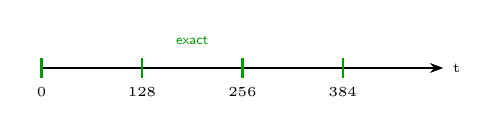
\begin{tikzpicture}[>=Stealth, scale=0.85]
  \draw[->] (0,0) -- (6,0) node[right]{\tiny t};
  \foreach \i/\lbl in {0/0, 1.5/128, 3/256, 4.5/384} {
    \draw[thick, green!60!black] (\i, -0.15) -- (\i, 0.15);
    \node[below, font=\tiny] at (\i, -0.15) {\lbl};
  }
  \node[above, font=\tiny\sffamily, green!60!black] at (2.25, 0.2) {exact};
\end{tikzpicture}
\end{center}
\end{column}

\begin{column}{0.48\textwidth}
\begin{lstlisting}[style=cstyle, title={Wrong: cumulative drift}]
void callback(void *ptr) {
    do_work();  /* takes ~3 ticks */
    /* start = now */
    tiku_timer_restart(&my_timer);
}

/* Ticks: 0, 131, 262, 393, ...
   Drifts by ~3 ticks each cycle */
\end{lstlisting}

\begin{center}
\begin{tikzpicture}[>=Stealth, scale=0.85]
  \draw[->] (0,0) -- (6,0) node[right]{\tiny t};
  \foreach \i/\lbl in {0/0, 1.55/131, 3.1/262, 4.7/393} {
    \draw[thick, red!70!black] (\i, -0.15) -- (\i, 0.15);
    \node[below, font=\tiny] at (\i, -0.15) {\lbl};
  }
  \node[above, font=\tiny\sffamily, red!70!black] at (2.3, 0.2) {drifts};
\end{tikzpicture}
\end{center}
\end{column}
\end{columns}
\end{frame}

% ===========================================================================
\section{File Organization}
% ===========================================================================

\begin{frame}[fragile]{Timer Module Files}
\begin{table}
\centering
\small
\begin{tabular}{@{}llp{5.5cm}@{}}
\toprule
\textbf{Layer} & \textbf{File} & \textbf{Role} \\
\midrule
\multirow{2}{*}{Clock}
  & \texttt{kernel/timers/tiku\_clock.h} & Clock API, types, macros \\
  & \texttt{kernel/timers/tiku\_clock.c} & Delegates to arch layer \\
\midrule
\multirow{2}{*}{Software Timer}
  & \texttt{kernel/timers/tiku\_timer.h} & Timer API (event + callback) \\
  & \texttt{kernel/timers/tiku\_timer.c} & Timer process, linked list \\
\midrule
\multirow{2}{*}{Hardware Timer}
  & \texttt{kernel/timers/tiku\_htimer.h} & htimer API (ISR-driven) \\
  & \texttt{kernel/timers/tiku\_htimer.c} & Singleton dispatch \\
\midrule
\multirow{4}{*}{Arch (MSP430)}
  & \texttt{arch/.../tiku\_timer\_arch.h}  & Clock config, tick rate \\
  & \texttt{arch/.../tiku\_timer\_arch.c}  & Timer A0 ISR, ACLK setup \\
  & \texttt{arch/.../tiku\_htimer\_arch.h} & htimer arch interface \\
  & \texttt{arch/.../tiku\_htimer\_arch.c} & Timer A1 ISR, scheduling \\
  & \texttt{arch/.../tiku\_htimer\_config.h} & Preset configurations \\
\midrule
Tests
  & \texttt{tests/test\_timer.c} & 6 test cases \\
\bottomrule
\end{tabular}
\end{table}
\end{frame}

% ===========================================================================
\section{Test Suite}
% ===========================================================================

\begin{frame}[fragile]{Test Configuration}
\begin{columns}[T]
\begin{column}{0.48\textwidth}
\begin{lstlisting}[style=cstyle, title={tests/tiku\_test\_config.h}]
#define TEST_ENABLE 1

/* Software timer tests */
#define TEST_TIMER           1
#define TEST_TIMER_EVENT     1
#define TEST_TIMER_CALLBACK  1
#define TEST_TIMER_PERIODIC  1
#define TEST_TIMER_STOP      1

/* Hardware timer tests */
#define TEST_HTIMER_BASIC    1
#define TEST_HTIMER_PERIODIC 1
\end{lstlisting}
\end{column}

\begin{column}{0.48\textwidth}
\textbf{Test constants:}
\begin{lstlisting}[style=cstyle]
/* 1 second */
#define TEST_TIMER_INTERVAL \
    TIKU_CLOCK_SECOND
/* 250 ms */
#define TEST_TIMER_SHORT \
    (TIKU_CLOCK_SECOND / 4)
/* Periodic repeat count */
#define TEST_TIMER_PERIODIC_CNT 3
/* htimer: 100 ms */
#define TEST_HTIMER_PERIOD \
    (TIKU_HTIMER_SECOND / 10)
/* htimer repeat count */
#define TEST_HTIMER_REPEAT_CNT 5
\end{lstlisting}
\end{column}
\end{columns}
\end{frame}

% ---------------------------------------------------------------------------
\begin{frame}{Test Cases Overview}
\begin{table}
\centering
\small
\begin{tabular}{@{}clp{7.5cm}@{}}
\toprule
\textbf{\#} & \textbf{Test Flag} & \textbf{What It Verifies} \\
\midrule
1 & \texttt{TEST\_TIMER\_EVENT}     & Event timer posts \texttt{TIKU\_EVENT\_TIMER} to process \\
2 & \texttt{TEST\_TIMER\_CALLBACK}  & Callback timer fires function; count == 1 \\
3 & \texttt{TEST\_TIMER\_PERIODIC}  & \texttt{tiku\_timer\_reset()} reschedules 3 times; drift-free \\
4 & \texttt{TEST\_TIMER\_STOP}      & \texttt{tiku\_timer\_stop()} cancels before expiration \\
5 & \texttt{TEST\_HTIMER\_BASIC}    & One-shot htimer fires ISR callback exactly once \\
6 & \texttt{TEST\_HTIMER\_PERIODIC} & Self-rescheduling htimer fires 5 times; drift-free \\
\bottomrule
\end{tabular}
\end{table}
\end{frame}

% ---------------------------------------------------------------------------
\begin{frame}[fragile]{Test Deep Dive: Event \& Callback}
\begin{columns}[T]
\begin{column}{0.48\textwidth}
\begin{lstlisting}[style=cstyle, title={Event timer test}]
static struct tiku_timer t;

TIKU_PROCESS_THREAD(test_ev, ev, data)
{
    TIKU_PROCESS_BEGIN();

    tiku_timer_set_event(&t,
        TEST_TIMER_INTERVAL);

    TIKU_PROCESS_WAIT_EVENT_UNTIL(
        ev == TIKU_EVENT_TIMER);

    TEST_ASSERT(
        tiku_timer_expired(&t));
    TEST_PASS("event timer OK");

    TIKU_PROCESS_END();
}
\end{lstlisting}
\end{column}

\begin{column}{0.48\textwidth}
\begin{lstlisting}[style=cstyle, title={Callback timer test}]
static struct tiku_timer t;
static volatile int cb_count = 0;

void test_cb(void *ptr) {
    cb_count++;
}

TIKU_PROCESS_THREAD(test_cb_proc,
    ev, data)
{
    TIKU_PROCESS_BEGIN();

    cb_count = 0;
    tiku_timer_set_callback(&t,
        TEST_TIMER_SHORT,
        test_cb, NULL);

    /* Wait past expiration */
    tiku_clock_wait(
        TEST_TIMER_SHORT * 2);

    TEST_ASSERT(cb_count == 1);
    TEST_PASS("callback OK");

    TIKU_PROCESS_END();
}
\end{lstlisting}
\end{column}
\end{columns}
\end{frame}

% ---------------------------------------------------------------------------
\begin{frame}[fragile]{Test Deep Dive: Periodic \& Stop}
\begin{columns}[T]
\begin{column}{0.48\textwidth}
\begin{lstlisting}[style=cstyle, title={Periodic callback test}]
static volatile int count = 0;

void periodic_cb(void *ptr) {
    count++;
    if (count < TEST_TIMER_PERIODIC_CNT)
        tiku_timer_reset(&t);
    /* else: don't reschedule */
}

/* After sufficient time: */
TEST_ASSERT(count == 3);
TEST_ASSERT(tiku_timer_expired(&t));
TEST_PASS("periodic OK");
\end{lstlisting}

Verifies:
\begin{itemize}
  \item Fires exactly 3 times
  \item \texttt{reset()} reschedules drift-free
  \item Timer expires when not rescheduled
\end{itemize}
\end{column}

\begin{column}{0.48\textwidth}
\begin{lstlisting}[style=cstyle, title={Timer stop test}]
static volatile int fired = 0;

void stop_cb(void *ptr) {
    fired++;
}

/* Set 1-second callback */
tiku_timer_set_callback(&t,
    TEST_TIMER_INTERVAL,
    stop_cb, NULL);

/* Stop before expiration */
tiku_timer_stop(&t);

/* Wait past original expiration */
tiku_clock_wait(
    TEST_TIMER_INTERVAL * 2);

TEST_ASSERT(fired == 0);
TEST_PASS("stop OK");
\end{lstlisting}

Verifies callback \textbf{never fires}
after \texttt{stop()}.
\end{column}
\end{columns}
\end{frame}

% ===========================================================================
\section{Summary}
% ===========================================================================

\begin{frame}{Summary}
\begin{columns}[T]
\begin{column}{0.48\textwidth}
\begin{block}{Three Timer Layers}
\begin{itemize}
  \item \textbf{System Clock}: 128\,Hz tick from 32.768\,kHz crystal
  \item \textbf{Software Timers}: event + callback modes, linked list, drift-free reset
  \item \textbf{Hardware Timer}: ISR-driven, 1\,$\mu$s resolution, singleton
\end{itemize}
\end{block}

\begin{block}{Key Design Choices}
\begin{itemize}
  \item Wraparound-safe 16-bit arithmetic
  \item Double-read for atomic counter access
  \item Timer process auto-cleans dead process timers
  \item Static allocation throughout
\end{itemize}
\end{block}
\end{column}

\begin{column}{0.48\textwidth}
\begin{block}{Configuration}
\begin{itemize}
  \item Tick rate: power-of-2 (default 128)
  \item htimer presets: high accuracy, balanced, low power, custom
  \item Per-subsystem debug flags
\end{itemize}
\end{block}

\begin{block}{Test Coverage}
6 tests: event timer, callback timer, periodic, stop, htimer one-shot, htimer periodic.
\end{block}
\end{column}
\end{columns}
\end{frame}

% ---------------------------------------------------------------------------
\begin{frame}{Thank You}
\begin{center}
\Large\textbf{TikuOS Timer Subsystem}\\[0.5em]
\normalsize Clock, Software Timers \& Hardware Timers for Physical AI Endpoints\\[1.5em]

\begin{tabular}{rl}
  Repository: & \url{https://github.com/tikuos/tikuOS} \\
  License:    & Apache 2.0 \\
  Clock:      & \texttt{kernel/timers/tiku\_clock.h} \\
  Timers:     & \texttt{kernel/timers/tiku\_timer.h} \\
  htimer:     & \texttt{kernel/timers/tiku\_htimer.h} \\
  Tests:      & \texttt{tests/test\_timer.c} \\
\end{tabular}
\end{center}
\end{frame}

\end{document}
